\section{Inferens baseret på polyeder lemmaet} \label{subsec:teste_polyhedron}
Variabeludvælgelsen af LARS og lasso kan karakteriseres som et polyeder jævnfør \citep{post_inference}, og derfor vil vi i dette afsnit betragte polyeder lemmaet, hvorudfra vi udfører inferens.
Lad os antage
\begin{align*}
\y \sim N \del{\tmu,  \boldsymbol{\Sigma}},
\end{align*}
hvor \(\tmu\) er en ukendt \(n \times 1\) vektor og \(\boldsymbol{\Sigma}\) er en kendt \(n \times n\) matrix.
Dette generaliserer vores setup i \eqref{eq:set-up}.
Betragt et polyeder
\begin{align*}
\mathcal{P} = \cbr{\y : \ \boldsymbol{\Gamma} \y \geq \mathbf{u}},
\end{align*}
hvor \(\boldsymbol{\Gamma}\) er en \(m \times n\) matrix, \(\mathbf{u}\) er en \(m \times 1\) vektor og uligheden skal fortolkes elementvis.

%Lasso løsningen for en fast værdi af \(\lambda\) er karakteriseret ved en mængde af aktive variable og fortegnene af deres koefficienter.
%Det viser sig at udvælgelsen af variable kan skrives på formen \(\cbr{\boldsymbol{\Gamma} \y \geq \mathbf{u}}\).
%Med andre ord svarer mængden \(\cbr{\y : \ \boldsymbol{\Gamma} \y \geq \mathbf{u}}\) til værdierne af \(\y\) som giver samme aktive variable og fortegn.
%Det samme gør sig gældende for LARS algoritmen efter \(k\) steps.

Lad \(\teta\) være en \(n \times 1\) vektor, da er målet at lave inferens om \(\teta^T \tmu\) givet \(\y \in \mathcal{P}\).
Vi betragter nulhypotesen \(\hyp_0 : \teta^T \tmu = 0\) givet \(\y \in \mathcal{P}\).
For \(\teta = \del{\X_{\A_k}^+}^T \mathbf{e}_k\), hvor \(\X_{\A_k}\) er en matrix, der består af de søjler i \(\X\), som svarer til prædiktorerne i \(\A_k\), \( \del{\X_{\A_k}^+} = \del{\X_{\A_k}^T \X_{\A_k}}^{-1} \X_{\A_k}^T\) er den pseudoinverse af \(\X_{\A_k}\) og \(\mathbf{e}_k\) er \(k\)'te standard enhedsvektor, har vi, at
\begin{align}
\teta^T \tmu = \mathbf{e}_k^T \X_{\A_k}^+ \tmu =  \mathbf{e}_k^T \del{\X_{\A_k}^T \X_{\A_k}}^{-1} \X_{\A_k}^T \X_{\A_k} \tbeta = \beta_k, \label{eq:tg_beta}
\end{align}
og nulhypotesen svarer derfor til at teste om koefficienten af den sidst tilføjede variabel, i regressionen af \(\tmu\) på \(\X_{\A_k}\), er lig 0.

%Vi antager, at kolonnerne af \(\X\) er i general position (se definition \ref{defn:general_position}), hvilket medfører at løsningsstierne for LARS og LARS med lasso modifikation er entydige \citep{lasso_unique}. 
%For kovarians testen antages at den sande model er lineær, dette er ikke nødvendigt for TG testen.
%
%TG testen antager ikke at den sande model er lineær, dvs vi antager ikke at \(\tmu = \X \tbeta^*\).
%

Nedenfor gives en alternativ repræsentation af \(\mathcal{P}\).
%
\begin{lem}[Polyeder lemma] \label{lem:polyhedral}
For ethvert \(\boldsymbol{\Sigma}\) og \(\teta\) hvor \(\teta^T \boldsymbol{\Sigma} \teta \neq 0\), gælder der, at
\begin{align}
\boldsymbol{\Gamma} \y \geq \mathbf{u} \ \Longleftrightarrow \ \mathcal{V}^- \del{\y} \leq \boldsymbol{\eta}^T \y \leq \mathcal{V}^+ \del{\y}, \quad \mathcal{V}^0 \del{\y} \leq 0, \label{eq:post_8}
\end{align}
hvor
\begin{align}
\mathcal{V}^- \del{\y} &= \max_{j: \rho_j > 0} \frac{u_j - \del{\boldsymbol{\Gamma} \y}_j + \rho_j \boldsymbol{\eta}^T \y}{\rho_j}, \label{eq:V-} \\
\mathcal{V}^+ \del{\y} &= \min_{j: \rho_j < 0} \frac{u_j - \del{\boldsymbol{\Gamma} \y}_j + \rho_j \boldsymbol{\eta}^T \y}{\rho_j}, \label{eq:V+} \\
\mathcal{V}^0 \del{\y} &= \max_{j: \rho_j = 0} u_j - \del{\boldsymbol{\Gamma} \y}_j, \label{eq:V0} 
\end{align}
og \(\boldsymbol{\rho}=\frac{\boldsymbol{\Gamma} \boldsymbol{\Sigma} \boldsymbol{\eta}}{\teta^T \boldsymbol{\Sigma} \teta}\).
Yderligere  er \(\boldsymbol{\eta}^T \y\) og \(\del{\mathcal{V}^-\del{\y}, \mathcal{V}^+\del{\y},\mathcal{V}^0\del{\y}}\) uafhængige. 
\end{lem}
%
\begin{proof}
Omskriv uligheden \(\boldsymbol{\Gamma} \y \geq \mathbf{u}\)
\begin{align*}
\boldsymbol{\Gamma} \del{ \frac{\boldsymbol{\Sigma} \boldsymbol{\eta} \teta^T}{\teta^T \boldsymbol{\Sigma} \teta} \y + \del{\mathbf{I}_n - \frac{\boldsymbol{\Sigma}\boldsymbol{\eta} \teta^T}{\teta^T \boldsymbol{\Sigma} \teta}} \y} \geq \mathbf{u}.
\end{align*}
Lad \(\boldsymbol{\rho} = \frac{\boldsymbol{\Gamma} \boldsymbol{\Sigma} \boldsymbol{\eta}}{\teta^T \boldsymbol{\Sigma} \teta}\), da fås, at
\begin{align*}
\boldsymbol{\rho} \teta^T \y + \boldsymbol{\Gamma} \y - \boldsymbol{\rho} \teta^T \y &\geq \mathbf{u} \\
\boldsymbol{\rho} \teta^T \y &\geq \mathbf{u} - \boldsymbol{\Gamma} \y + \boldsymbol{\rho} \teta^T \y,
\end{align*}
som kan udtrykkes som
\begin{align*}
\teta^T \y & \geq \frac{u_j - \del{\boldsymbol{\Gamma} \y}_j + \rho_j \boldsymbol{\eta}^T \y}{\rho_j}, \quad \text{for } \rho_j > 0, \\
\teta^T \y & \leq \frac{u_j - \del{\boldsymbol{\Gamma} \y}_j + \rho_j \boldsymbol{\eta}^T \y}{\rho_j}, \quad \text{for } \rho_j < 0, \\
0 &\geq u_j - \del{\boldsymbol{\Gamma} \y}_j, \quad \text{for } \rho_j < 0,
\end{align*}
eller
\begin{align*}
\teta^T \y & \geq \mathcal{V}^- \del{\y} = \max_{j: \rho_j > 0} \frac{u_j - \del{\boldsymbol{\Gamma} \y}_j + \rho_j \boldsymbol{\eta}^T \y}{\rho_j},\\
\teta^T \y & \leq \mathcal{V}^+ \del{\y} = \min_{j: \rho_j < 0} \frac{u_j - \del{\boldsymbol{\Gamma} \y}_j + \rho_j \boldsymbol{\eta}^T \y}{\rho_j}, \\
0 &\geq \mathcal{V}^0 \del{\y} = \max_{j: \rho_j = 0} u_j - \del{\boldsymbol{\Gamma} \y}_j.
\end{align*}
Uafhængigheden mellem \(\del{\mathcal{V}^-\del{\y}, \mathcal{V}^+\del{\y},\mathcal{V}^0\del{\y}}\) og \(\boldsymbol{\eta}^T \y\), kommer af, at \(\mathcal{V}^-, \mathcal{V}^+\) og \(\mathcal{V}^0\) er funktioner af \(\y - \frac{ \boldsymbol{\Sigma} \boldsymbol{\eta} \boldsymbol{\eta}^T \y}{\teta^T \boldsymbol{\Sigma} \teta} \), som under antagelsen \(\y \sim N \del{\tmu,  \boldsymbol{\Sigma}}\) er uafhængig af \(\teta^T \y\).
\end{proof}
%
Resultatet i \eqref{eq:post_8} er deterministisk og gælder for alle \(\y\).
Kun uafhængighedsresultatet afhænger af normaliteten af \(\y\).
Se figur \ref{fig:polyhedron} for en geometrisk illustration af lemmaet.
Intuitivt kan resultatet forklares som følgende, hvor vi antager for nemheds skyld, at \(\boldsymbol{\Sigma}= \mathbf{I}_n\).
Først dekomponeres \(\y=P_{\boldsymbol{\eta}} \y + P_{\boldsymbol{\eta}^\perp} \y\), hvor \(P_{\boldsymbol{\eta}} \y = \frac{\boldsymbol{\eta} \boldsymbol{\eta}^T \y}{\Vert \boldsymbol{\eta} \Vert_2^2}\) er projektionen af \(\y\) langs \(\boldsymbol{\eta}\) og \(P_{\boldsymbol{\eta}^\perp} \y = \y - P_{\boldsymbol{\eta}} \y\) er projektionen på det ortogonale komplement af \(\boldsymbol{\eta}\).
Vi kan betragte \(\y\) som en afvigelse fra \(P_{\boldsymbol{\eta}^\perp} \y\) af størrelsen \(\boldsymbol{\eta}^T \y\) langs linjen bestemt af \(\boldsymbol{\eta}\).
Størrelserne \(\mathcal{V}^-\) og \(\mathcal{V}^+\) bestemmer, hvor langt vi kan afvige på hver side af \(P_{\boldsymbol{\eta}^\perp} \y\), inden \(\y\) forlader polyederet, hvoraf vi får uligheden \(\mathcal{V}^- \leq \boldsymbol{\eta}^T \y \leq \mathcal{V}^+\).
Nogle flader af polyederet kan være perfekt justeret med \(\boldsymbol{\eta}\), dvs deres normalvektorer kan være ortogonale med \(\boldsymbol{\eta}\).
Dette kan tjekkes ud fra \(\mathcal{V}^0\) ved at \(\y\) ligger på den rigtige side af disse flader.  
%
\begin{figure}[H]
\centering
\scalebox{1}{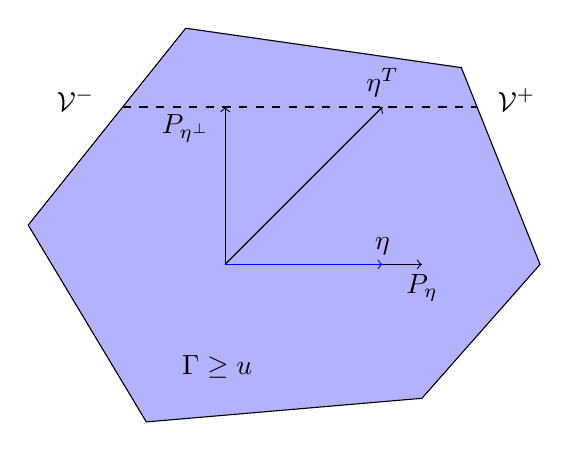
\begin{tikzpicture}
\draw (-1,-2) -- (-2.5,0.5) -- (-0.5,3)-- (3,2.5) -- (4,0) -- (2.5,-1.7) -- (-1,-2)[fill = blue!30];
\draw [<-] (0,2) node [label={[xshift=-0.5cm, yshift=-0.7cm]$P_{\boldsymbol{\eta}^\perp} \y$}] {} -- (0,0);
\draw[<-] (2.5,0) node [below] {$P_{\boldsymbol{\eta}} \y$} -- (0,0);
\draw[<-][blue] (2,0) node [black, above] {$\boldsymbol{\eta}$} -- (0,0);
\draw[<-] (2,2) node [above] {$\boldsymbol{\eta}^T \y$} -- (0,0) node [label={[xshift=1.7cm, yshift=1cm]$\y$}] {};
\draw[dashed] (-1.3,2) node [label={[xshift=-0.6cm, yshift=-0.3cm]$\mathcal{V}^- \del{\y}$}] {} -- (3.2,2) node [label={[xshift=0.5cm, yshift=-0.3cm]$\mathcal{V}^+ \del{\y}$}] {};
\draw node [label={[xshift=-0.1cm, yshift=-1.7cm]$\cbr{\Gamma \y \geq u}$}] {};
\end{tikzpicture}}
\caption{Illustration af polyeder lemmaet for \(p=2\). For simplicitet antages at \(\boldsymbol{\Sigma} = \mathbf{I}_n\). Det blå område er polyederet \(\cbr{\y : \ \boldsymbol{\Gamma} \y \geq \mathbf{u}}\).
Ved at dekomponere \(\y\) til dens projektion på \(\teta\) og dens projektion på det ortogonale komplement af \(\teta\), ses at \(\boldsymbol{\Gamma} \y \geq \mathbf{u}\) er opfyldt, hvis og kun hvis \(\teta^T \y\) ikke afviger for langt fra \(P_{\boldsymbol{\eta}^\perp} \y\), dvs den skal fastholdes imellem grænserne \(\mathcal{V}^-\) og \(\mathcal{V}^+\).
Yderligere er grænserne \(\mathcal{V}^-\) og \(\mathcal{V}^+\) kun funktioner af \(P_{\boldsymbol{\eta}^\perp} \y\), derfor er de uafhængige af \(\teta^T \y\) under normalitet.} \label{fig:polyhedron}
\end{figure}
%
Af lemma \ref{lem:polyhedral} kan fordelingen af enhver lineær funktion \(\boldsymbol{\eta}^T \y\) givet \(\boldsymbol{\Gamma} \y \geq \mathbf{u}\) skrives som følgende betinget fordeling
\begin{align*}
\boldsymbol{\eta}^T \y \given \mathcal{V}^- \del{\y} \leq \boldsymbol{\eta}^T \y \leq \mathcal{V}^+ \del{\y}, \quad \mathcal{V}^0 \del{\y} \leq 0.
\end{align*}
Da \(\boldsymbol{\eta}^T \y\) er normalfordelt, er ovenstående trunkeret normalfordelt.
%
\begin{lem}  \label{lem:lem2}
Lad \(\Phi \del{x}\) betegne fordelingsfunktionen af en standard normalfordeling, da er fordelingsfunktionen af en trunkeret normalfordelt stokastisk variabel med middelværdi \(\mu\) og varians \(\sigma^2\) indenfor intervallet \(\sbr{a,b}\) givet ved
\begin{align*}
F_{\mu, \sigma^2}^{\sbr{a,b}} \del{x} = \frac{\Phi\del{\frac{x-\mu}{\sigma}} - \Phi\del{\frac{a-\mu}{\sigma}}}{\Phi\del{\frac{b-\mu}{\sigma}} - \Phi\del{\frac{a-\mu}{\sigma}}}.
\end{align*}
Hvis \(\boldsymbol{\eta}^T \boldsymbol{\Sigma} \boldsymbol{\eta} \neq 0\), da er \(F_{\boldsymbol{\eta}^T \tmu, \boldsymbol{\eta}^T \boldsymbol{\Sigma} \boldsymbol{\eta}}^{\sbr{\mathcal{V}^-,\mathcal{V}^+}} \del{\boldsymbol{\eta}^T \y} \) givet \(\boldsymbol{\Gamma} \y \geq \mathbf{u}\) en standard uniform fordeling, dvs
\begin{align*}
\mathbb{P} \del{F_{\boldsymbol{\eta}^T \tmu, \boldsymbol{\eta}^T \boldsymbol{\Sigma} \boldsymbol{\eta}}^{\sbr{\mathcal{V}^-,\mathcal{V}^+}} \del{\boldsymbol{\eta}^T \y} \leq \alpha \given \boldsymbol{\Gamma} \y \geq \mathbf{u}} = \alpha, 
\end{align*}
for ethvert \(0 \leq \alpha \leq 1\), hvor \(\mathcal{V}^-\) og \(\mathcal{V}^+\) er defineret i \eqref{eq:V-} samt \eqref{eq:V+}. 
\end{lem}
%
\begin{proof}
Hvis \(Z \sim N \del{\mu, \sigma^2}\) og trunkeret i intervallet \(\sbr{a,b}\) og \(F_{\mu, \sigma^2}^{\sbr{a,b}} \del{Z}\) er dens fordelingsfunktion, da er \(F_{\mu, \sigma^2}^{\sbr{a,b}} \del{Z} \sim \text{unif} \del{0,1}\).
Heraf følger det, at
\begin{align*}
\mathbb{P} \del{F_{\boldsymbol{\eta}^T \tmu, \boldsymbol{\eta}^T \boldsymbol{\Sigma} \boldsymbol{\eta}}^{\sbr{a,b}} \del{\boldsymbol{\eta}^T \y} \leq \alpha \given \teta^L \leq \teta \leq \teta^U} = \alpha, 
\end{align*}
for ethvert  \(0 \leq \alpha \leq 1\) og faste grænser \(\teta^L\), \(\teta^U\).
Hvis vi integrerer over \(\mathcal{V}^- = \teta^L\), \(\mathcal{V}^+ = \teta^U\) og \(\mathcal{V}^0 \leq 0\) og anvender, at \(\teta^T \y\) og \(\del{\mathcal{V}^-\del{\y}, \mathcal{V}^+\del{\y},\mathcal{V}^0\del{\y}}\) er uafhængige fra lemma \ref{lem:polyhedral}, får vi resultatet i lemma \ref{lem:lem2}.
\end{proof}
Lemma \ref{lem:lem2} anvendes til at lave betinget inferens af enhver lineær funktion \(\boldsymbol{\eta}^T \boldsymbol{\mu}\).
Vi kan udregne \(p\)-værdier for nulhypotesen \(\hyp_0: \boldsymbol{\eta}^T \boldsymbol{\mu}=0\) og tilhørende betingede konfidensintervaller for \(\boldsymbol{\eta}^T \tmu\).

Herefter betragtes enkelt- og dobbeltsidet inferens.
%
\begin{lem}[Enkeltsidet betinget inferens efter variabeludvælgelsen] \label{lem:lem3}
Givet \(\boldsymbol{\eta}^T \Sigma \boldsymbol{\eta} \neq 0\), antag at vi vil teste
\begin{align*}
\hyp_0: \boldsymbol{\eta}^T \tmu=0 \quad \text{imod} \quad \hyp_1: \boldsymbol{\eta}^T \tmu > 0.
\end{align*}
Definer teststørrelsen
\begin{align}
T=1- F_{0, \boldsymbol{\eta}^T \boldsymbol{\Sigma} \boldsymbol{\eta}}^{\sbr{\mathcal{V}^-, \mathcal{V}^+}} \del{\boldsymbol{\eta}^T \y}, \label{eq:post_1.14}
\end{align}
hvor fordelingsfunktionen af \(\boldsymbol{\eta}^T \y \sim N \del{0,  \boldsymbol{\eta}^T \boldsymbol{\Sigma} \boldsymbol{\eta}}\) i intervallet \(\sbr{\mathcal{V}^-, \mathcal{V}^+}\) er givet i lemma \ref{lem:lem2}.
Teststørrelsen \(T\) er da \(p\)-værdien for \(\hyp_0\) givet \(\boldsymbol{\Gamma} \y \geq \mathbf{u}\)
\begin{align}
\mathbb{P}_{\boldsymbol{\eta}^T \tmu=0} \del{T \leq \alpha \given \boldsymbol{\Gamma }\y \geq \mathbf{u}} = \alpha, \label{eq:post_1.15}
\end{align}
for ethvert \(0 \leq \alpha \leq 1\). 
Endvidere, definer \(\delta_{\alpha}\) ved
\begin{align}
1-F_{\delta_{\alpha}, \boldsymbol{\eta}^T \Sigma \boldsymbol{\eta}}^{\sbr{\mathcal{V}^-, \mathcal{V}^+}} \del{\boldsymbol{\eta}^T \y} &= \alpha. \label{eq:post_1.16}
\end{align}
Da er \(I= [\delta_\alpha, \infty )\) et enkeltsidet konfidensinterval for \(\teta^T \tmu\) givet \(\boldsymbol{\Gamma} \y \geq \mathbf{u}\)
\begin{align}
\mathbb{P} \del{\boldsymbol{\eta}^T \tmu \geq \delta_\alpha \given \boldsymbol{\Gamma} \y \geq \mathbf{u}} = 1- \alpha. \label{eq:post_1.17}
\end{align}
\end{lem}
%
Vi har styrke imod den enkeltsidede alternativ hypotese \(\hyp_1 : \teta^T \tmu > 0\), da \(1-F_{\mu, \sigma^2}^{\sbr{a,b}} \del{x}\), evalueret i ethvert fast punkt \(x\), er monotont stigende i \(\mu\).
Dette gælder også for konfidensintervallet i \eqref{eq:post_1.16} og \eqref{eq:post_1.17}.
Herefter betragtes dobbeltsidet inferens.
%
\begin{lem}[Dobbeltsidet betinget inferens efter variabeludvælgelsen] \label{lem:lem4}
Givet \(\boldsymbol{\eta}^T \boldsymbol{\Sigma} \boldsymbol{\eta} \neq 0\), antag at vi vil teste
\begin{align*}
\hyp_0: \boldsymbol{\eta}^T \tmu=0 \quad \text{imod} \quad \hyp_1: \boldsymbol{\eta}^T \tmu \neq 0.
\end{align*}
Definer teststørrelsen
\begin{align}
T=2 \cdot \min\cbr{F_{0, \boldsymbol{\eta}^T \boldsymbol{\Sigma} \boldsymbol{\eta}}^{\sbr{\mathcal{V}^-, \mathcal{V}^+}} \del{\boldsymbol{\eta}^T \y}, 1 - F_{0, \boldsymbol{\eta}^T \boldsymbol{\Sigma} \boldsymbol{\eta}}^{\sbr{\mathcal{V}^-, \mathcal{V}^+}} \del{\boldsymbol{\eta}^T \y}}, \label{eq:post_1.18}
\end{align}
hvor fordelingsfunktionen af \(\boldsymbol{\eta}^T \y \sim N \del{0,  \boldsymbol{\eta}^T \boldsymbol{\Sigma} \boldsymbol{\eta}}\) i intervallet \(\sbr{\mathcal{V}^-, \mathcal{V}^+}\) er givet i lemma \ref{lem:lem2}.
Teststørrelsen \(T\) er da \(p\)-værdien for \(\hyp_0\) givet \(\boldsymbol{\Gamma} \y \geq \mathbf{u}\)
\begin{align}
\mathbb{P}_{\boldsymbol{\eta}^T \tmu=0} \del{T \leq \alpha \given \boldsymbol{\Gamma} \y \geq \mathbf{u}} = \alpha, \label{eq:post_1.19}
\end{align}
for ethvert \(0 \leq \alpha \leq 1\). 
Definer \(\delta_{\frac{\alpha}{2}}, \delta_{1-\frac{\alpha}{2}}\) som opfylder, at
\begin{align}
1-F_{\delta_{\frac{\alpha}{2}}, \boldsymbol{\eta}^T \boldsymbol{\Sigma} \boldsymbol{\eta}}^{\sbr{\mathcal{V}^-, \mathcal{V}^+}} \del{\boldsymbol{\eta}^T \y} &= \frac{\alpha}{2}, \label{eq:post_20} \\
1-F_{\delta_{1-\frac{\alpha}{2}}, \boldsymbol{\eta}^T \boldsymbol{\Sigma} \boldsymbol{\eta} }^{\sbr{\mathcal{V}^-, \mathcal{V}^+}} \del{\boldsymbol{\eta}^T \y} &= 1-\frac{\alpha}{2}. \label{eq:post_21}
\end{align}
Da gælder, at
\begin{align}
\mathbb{P} \del{\delta_{\frac{\alpha}{2}} \leq  \boldsymbol{\eta}^T \tmu \leq \delta_{1-\frac{\alpha}{2}} \given \boldsymbol{\Gamma} \y \geq \mathbf{u}} = 1- \alpha. \label{eq:post_22}
\end{align}
\end{lem}
%
Teststørrelsen i \eqref{eq:post_1.18}, defineret som 2 gange minimum af fordelingsfunktionen  og overlevelsesfunktionen, har styrke imod den alternative hypotese \(\hyp_1: \boldsymbol{\eta}^T \tmu \neq 0\).
Beviset for dens fordeling under nulhypotesen i \eqref{eq:post_1.19} kommer af, at hvis \(U\) følger en standard uniform fordeling, da gør \(2 \cdot \min \cbr{U,1-U}\) også.
Konstruktionen af konfidensintervallet i \eqref{eq:post_20}, \eqref{eq:post_21} og \eqref{eq:post_22} anvender igen monotonicitet af en trunkeret normal overlevelsesfunktion i den underliggende middelværdi parameter.

%Herefter vil vi vise at modeludvælgelsen for LARS og LARS med lasso modifikation kan karakteriseres som et polyhedron på formen \(\cbr{\y : \ \Gamma \y \geq 0}\).
%Efter dette beskrives formene af de eksakte betinget tests og intervaller, som er givet i lemma \ref{lem:polyhedral}-\ref{lem:lem4} for LARS og lasso.
%APPENDIKS

\subsection{TG testen}
Vi antager, at kolonnerne af \(\X\) er i general position, således at løsningsstierne for LARS og lasso er entydige \citep{lasso_unique}. 
Givet antallet af trin \(k\), da kan vi let udregne betingede \(p\)-værdier og konfidensintervaller, efter vi har konstrueret matricen \(\boldsymbol{\Gamma}\) for henholdsvis LARS eller lasso.
Lad os teste nulhypotesen \(\hyp_0: \ \teta^T \tmu = 0\), hvor \(\teta\) er arbitrær.

Som specificeret i lemma \ref{lem:polyhedral} udregnes størrelserne
\begin{align*}
\mathcal{V}^- \del{\y} &=  \max_{j: \rho_j > 0} \frac{- \del{\boldsymbol{\Gamma} \y}_j}{\rho_j} + \boldsymbol{\eta}^T \y = \max_{j: \del{\boldsymbol{\Gamma} \teta}_j > 0} - \del{\Gamma \y}_j \cdot \frac{\Vert \teta \Vert_2^2}{\del{\boldsymbol{\Gamma} \teta}_j} + \teta^T \y, \\
\mathcal{V}^+ \del{\y} &=\min_{j: \del{\boldsymbol{\Gamma} \teta}_j < 0} - \del{\Gamma \y}_j \cdot \frac{\Vert \teta \Vert_2^2}{\del{\Gamma \teta}_j} + \teta^T \y.
\end{align*}
%Antallet af operationer som kræves for at udregne \(\mathcal{V}^-\) og \(\mathcal{V}^+\) er \(O \del{mn}\), hvor \(m\) er antallet af rækker i \(\boldsymbol{\Gamma}\).
%
For at teste imod en enkeltsidet alternativ hypotese \(\hyp_1: \ \teta^T \tmu > 0\),  defineres teststørrelsen
\begin{align*}
T_k^\text{tg}=1- F_{0, \sigma^2 \Vert \boldsymbol{\eta} \Vert_2^2}^{\sbr{\mathcal{V}^-, \mathcal{V}^+}} \del{\boldsymbol{\eta}^T \y} = \frac{\Phi \del{\frac{\mathcal{V}^+}{\sigma \Vert \boldsymbol{\eta} \Vert_2}}-\Phi \del{\frac{\boldsymbol{\eta}^T \y}{\sigma  \Vert \boldsymbol{\eta} \Vert_2}}}{\Phi \del{\frac{\mathcal{V}^+}{\sigma  \Vert \boldsymbol{\eta} \Vert_2}}-\Phi \del{\frac{\mathcal{V}^-}{\sigma \Vert \boldsymbol{\eta} \Vert_2}}}.
\end{align*}
Af lemma \ref{lem:lem3} giver dette \(p\)-værdien givet udvælgelsen, dvs
\begin{align}
\mathbb{P}_{\boldsymbol{\eta}^T \tmu = 0} \del{T_k^\text{tg} \leq \alpha \given \widehat{\A}_k \del{\y} = \A_k, \widehat{s}_{\A_k} \del{y} = s_{\A_k}} = \alpha, \label{eq:post_32}
\end{align}
for ethvert \(0 \leq \alpha \leq 1\).
Vi definer  \(\delta_\alpha\) ved \(1-F_{\delta_{\alpha}, \sigma^2 \Vert \boldsymbol{\eta} \Vert_2^2}^{\sbr{\mathcal{V}^- \mathcal{V}^+}} \del{\boldsymbol{\eta}^T \y} = \alpha\).
Vi lader \(I_k = [\delta_\alpha, \infty)\), hvoraf vi får et enkeltsidet konfidensinterval
\begin{align}
\mathbb{P} \del{\boldsymbol{\eta}^T \tmu \in I_k \given \widehat{\A}_k \del{\y} = \A_k, \widehat{s}_{\A_k} \del{\y} = s_{\A_k}} = 1-\alpha. \label{eq:post_33}
\end{align}
For at teste imod en dobbeltsidet alternativ hypotese \(\hyp_1: \ \teta^T \tmu \neq 0\), betragtes teststørrelsen
\begin{align*}
T_k^\text{TG}= 2 \cdot \min \cbr{T_k^{\text{tg}}, 1-T_k^{\text{tg}}}.
\end{align*}
Af lemma \ref{lem:lem4} fås samme resultaterne i \eqref{eq:post_32} og \eqref{eq:post_33}, men hvor \(T_k^\text{tg}\) erstattes med \(T_k^\text{TG}\) og \(I_k\) erstattes med \(I_k'= \sbr{\delta_{\frac{\alpha}{2}}, \delta_{1-\frac{\alpha}{2}}}\).

For \(\teta = \del{\X_{\A_k}^+}^T \mathbf{e}_k\) er det enkeltsidede setup givet ved \(\hyp_0: \teta^T \tmu = 0\) og  \(\hyp_1: \teta^T \tmu > 0\), som ikke giver mening, da der ikke er grund til at tro at \(k\)'te regressionskoefficient \(\mathbf{e}_k^T \X_{\A_k}^+ \boldsymbol{\mu}\) skal være positiv.
Definer istedet \(\teta = s_k \del{\X_{\A_k}^+}^T \mathbf{e}_k\), hvor \(s_k\) er fortegnet af \(k\)'te variabel når den medtages i LARS eller lasso modellen, da er nulhypotesen \(\hyp_0: s_k \mathbf{e}_k^T \X_{\A_k}^+ \tmu = 0\) uændret, men den alternative hypotese \(\hyp_1: s_k \mathbf{e}_k^T \X_{\A_k}^+ \tmu > 0\) har nu en konkret fortolkning.
Den siger, at regressionskoefficienten af den sidst valgte variabel er ikke-nul og har samme fortegn som koefficienten i den fittede model.